\chapter{Potential Leakage Sources}

In this chapter, we discuss the potential leakage sources in the environment we have set up in \Cref{Chp: Experiment Setup}. 

\section{Subject} \label{Sec: Subjects}

Without loss of generality, in this report, we are interested in leakages with respect to the following subjects:

\begin{itemize}
	\item Content and size of encrypted data
	\item Cryptographic key materials
	\item Network topology
\end{itemize}

In this chapter we give a theoretical analysis of the exploitable side channel information in the WSN traffic. The inspection of protocol and implementation flaws are included in later chapters.

\section{Observables} \label{Sec: Observables}

As we have explained in \Cref{Chp: Experiment Setup}, we assumed the adversary has full access to all traffic being transmitted in the WSN. 

\begin{figure*}[th!]
	\center
	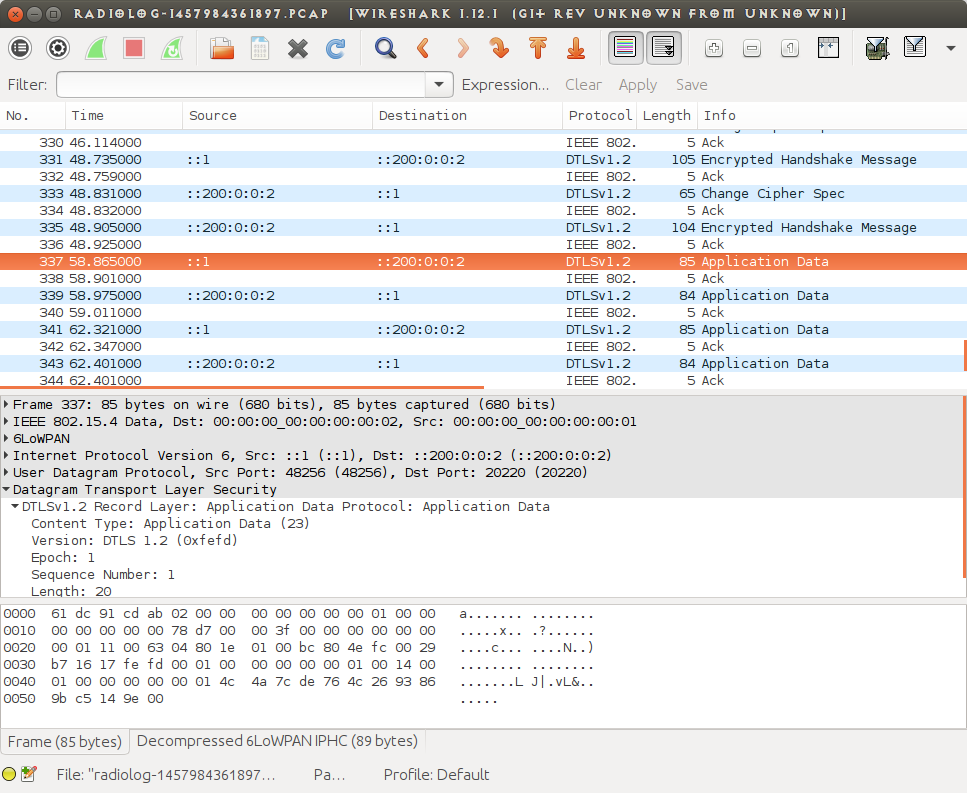
\includegraphics[width=0.9\textwidth]{fig/udpexample.png}
	\caption{An Example of Captured Traffic}
	\label{Fig: An Example of Captured Traffic}
\end{figure*}

\Cref{Fig: An Example of Captured Traffic} shows the packets captured in a Cooja experiment, analysed by Wireshark\cite{Wireshark}. In this research, we assume the value of ciphertext is independent to the plaintext and key. The following side channel information are available in the captured traffic shown in \Cref{Fig: An Example of Captured Traffic}:

\begin{description}[style=nextline]
	\item[Timing]
	Time of each packet sent is shown at the Time column on the upper half of \Cref{Fig: An Example of Captured Traffic}.
	\item[Packet Size]
	Packet size is shown in the Length column in the upper half of \Cref{Fig: An Example of Captured Traffic}.
	\item[Unencrypted headers]
	This is shown in the bottom half of \Cref{Fig: An Example of Captured Traffic}. The highlighted packet is a DTLS Data Record. We can see that the available headers are physical information (Frame), 802.15.4 MAC Header (IEEE 802.15.4 Data), compressed IPv6 Header (6LoWPAN and Internet Protocol Version 6), UDP Header (User Datagram Protocol) and DTLS Header (Datagram Transport Layer Security). Details of headers are shown under each tab.
\end{description}

Timing and packet size are always available in the captured traffic. The unencrypted headers depend on the security measure being used, which we explain in later sections.

Practically, the Receive Signal Strength Indicator, RSSI, should also be considered visible to the adversary. RSSI represents the RF signal strength. By measuring the RSSI of frames sent from a specific MAC source address,  it is possible for the adversary to reveal the geographical information of a specific Sensor Node. However we do not consider RSSI in this report as its physical character is beyond the scope of this report. Instead, we assume the adversary has prior knowledge of all geographic information of Sensor Nodes in the WSN.

\section{Packet Traces} \label{Sec: Packet Traces}

In this section, we explain some features of WSN traffic traces comparing to Internet applications.

Design of WSN applications tends to be simple and stateless due to the nature of constrained resources and unreliable transmission. As a result, data exchange is minimised for efficiency and robustness. From this aspect, we argue that our sample applications have captured these most significant characteristics of WSN applications.

In this report, we define a generic model for the data exchanging process in WSN applications.

\begin{definition} \label{Def: Session}
A Session is defined as a series of events where a Sensor Node reports application data to a Manager. A Session includes an optional Request sent from Manager to Sensor Node, and a Response containing the requested data sent from Sensor Node to Manager.
\end{definition}

\Cref{Fig: Overview of Session} shows an overview of a Session. Practically, the Manager can be a specific Sensor Node in the WSN, or a desktop connected to the WSN through a border router.

\begin{figure*}[th!]
	\center
	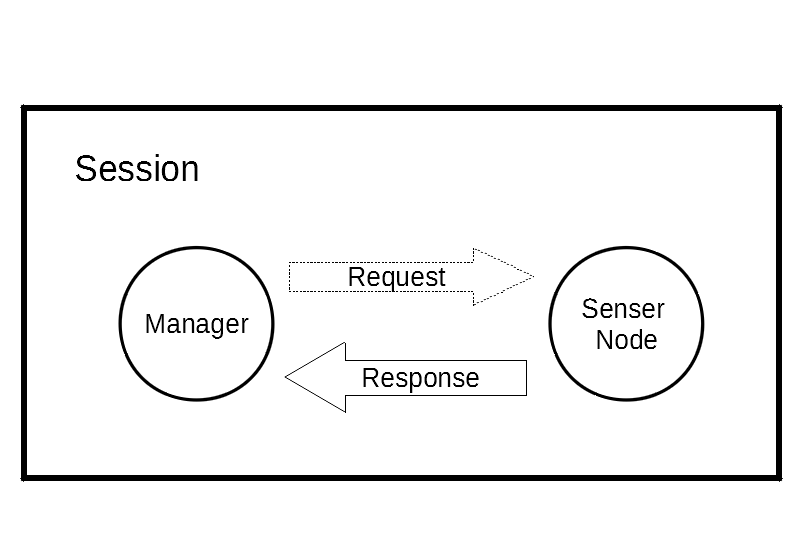
\includegraphics[width=0.8\textwidth]{fig/Session.png}
	\caption{Overview of Session}
	\label{Fig: Overview of Session}
\end{figure*}

\begin{definition} \label{Def: Trace}
A trace is all captured packets within one Session.
\end{definition}

Although not necessary under \Cref{Def: Session}, in most of our applications, there are typically one or two packets in a trace. The first one corresponds to Request and the second corresponds to Response. In some applications such as broadcast keyllsec or a CoAP application using OBSERVE option, there might be only one Response packet in a trace without a Request. In real world applications there might even be a Request without a Response, e.g. a command to control a light bulb. However, in this report, we define there is at least one packet corresponds to Response. We further assume the adversary is aware of the application running on the Sensor Nodes. Consequently, the adversary in our setting is able to distinguish a Request and a Response, but has no knowledge of the application data being transmitted within them.

We also assume the adversary is capable to distinguish Sessions. Practically, the time interval of packets within the same Session are usually significantly less then the interval between Sessions. \Cref{Fig: Example Traces of keyllsec} shows an example of traces in a unicast keyllsec application instance. Marked are packets from two continuous Sessions, where No.977 and No.990 are from the first Session and No.998 and No.1011 are from the second. We can see that the time interval within a Session is about 150ms which is significantly less than the 15s interval between Sessions.

\begin{figure*}[th!]
	\center
	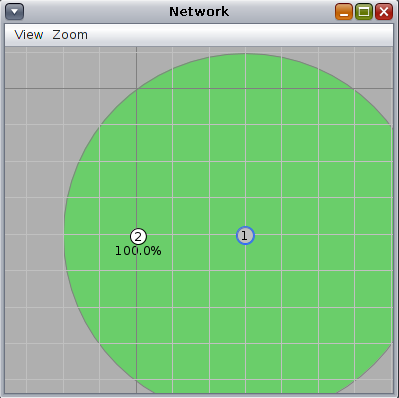
\includegraphics[width=0.5\textwidth]{fig/unicast_keyllsec.png}
	\\
	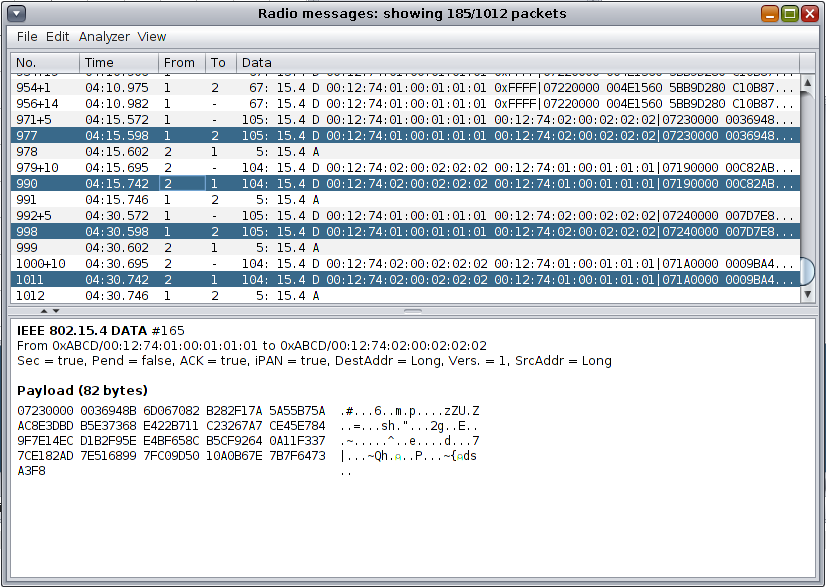
\includegraphics[width=0.9\textwidth]{fig/trace_keyllsec.png}
	\caption{
		Example Traces of keyllsec, \textcircled{1} is the sender and \textcircled{2} the receiver.
	}
	\label{Fig: Example Traces of keyllsec}
\end{figure*}

%The following paragraph is removed as the focus is shifted from application data to RPL messages.
%In this project, we consider only information leakage within one Session. Arguably, there could potential leakage when jointly analyse traces from different Sessions, e.g. the frequency of Requests can ``leak'' itself. However, we omit such leakage for generality as exploiting them requires further assumptions to the higher level application. Each Session in this report is also considered to be independent based on that fact that each execution of our code is independent to its last execution.

%Further more, in our applications the content of Request is a constant 3 bytes ASCII string ``GET''. We assume this known by the adversary. We make this assumption to focus on the leakage of the Application Data in Responses. 

\section{Theoretical Analysis} \label{Sec: Theoretical Analysis}

In this section we provide a theoretical analysis over all observables we explained in \Cref{Sec: Observables}. It is done in two approaches:

\begin{enumerate}
	\item Cross reference the observables with the exploited side channel information we introduced in \Cref{Sec: Traffic Analysis Attacks}
	\item Semantically analyse the observables. 
\end{enumerate}

%We discuss only the leakage over the attributes we specified in \Cref{Sec: A Review of Review}.

For some observables, we claim:

\begin{theorem} \label{Te: IR}
Under the leakage definitions of Mutual Information and g-leakage in \Cref{Subsec: Information Theory}, if an observable $Y$ is independent to a secret $X$, then there is $0$ leakage of $X$ over $Y$.
\end{theorem}

\Cref{Te: IR} intuitively holds. A formal proof is given in \Cref{Prf: IR}.

\begin{corollary} \label{Cor: Constant Leakage}
	An observable $Y$ with a constant value has no leakage under the leakage definitions of  Mutual Information and g-leakage in \Cref{Subsec: Information Theory}.
\end{corollary}

\begin{proof}
	This directly followed by the fact that a constant $y \in Y$ with $P(y) = 1$ is independent to the secret $X$.
\end{proof}

\subsection{Cross Reference of Observables with Known Attacks} \label{Subsec: Cross Reference}

Among all packet features we summarised in \Cref{Tbl: Classifiers in Traffic Analysis Literatures}, we only found four applicable in our WSN setting:
\begin{itemize}
	\item Packet size
	\item Total bytes
	\item Total Time (only for two packets Session)
	\item Total Per-direction Bandwidth
\end{itemize}

All other features have reduced to a constant or not applicable in our settings. The detailed analysis is described in \Cref{Detail Cross Reference}.

\subsection{Semantic Analysis}

In this section, we analysis the observables in \Cref{Sec: Observables} based on their semantics. The contents of headers can be referred to \Cref{Chp: Building Blocks}.

\subsubsection{Packet Size} \label{Semantic Packet Size}

%Linear relationship of length
We noticed that both noncoresec and DTLS use AES-128 with CCM mode to encrypt their payload. The data is therefore not padded due to the nature of a stream cipher. This effectively indicates that the length of a plaintext $l_P$ is expected to be linear to the length of its corresponding ciphertext $l_C$:

\begin{equation} \label{Eq: Linear Length}
	l_{C} = l_{P} + b
\end{equation}

where $b$ is a predictable constant induced by security measures such as MIC and additional headers.

Practically when the security measure increases the packet size to a value exceeding MTU, the packet will be immediately dropped. We assume plaintext is always in a reasonable length that does not result into a ciphertext exceeding MTU; otherwise the packets cannot be sent and the WSN loses its functionality.

From a leakage perspective, it is obvious that all bits of $l_P$ is leaked by $l_C$. A formal quantification of this leakage is given in \Cref{Linear Leakage}.

\subsubsection{Timing}

Timing information is another important side channel information in WSN traffic. Comparing to Internet applications, we consider timing information as a even more crucial leakage source in WSN for two reasons:

\begin{enumerate}
	\item The timing can be measured more accurately in WSN. Packet traces on Internet are usually measured at one side of the communication where the noise induced by RTT must be considered, whilst timing of every packet forwarding is known in our setup.
	\item The low performance of the WSN devices potentially increases the resolution of timing information. Any differences of execution time will be more distinguishable on these devices comparing to Internet servers.
\end{enumerate}

However, timing information would be hard to exploit without precise knowledge of the code running on the target Sensor Node. Several protocols may also affect the measurement, .e.g. ContikiMAC can change the behaviour of RF transmission and therefore additional preprocessing is required to measure the exact packet timing when it is used.

\subsubsection{Unencrypted Headers with noncoresec}

When noncoresec is enabled, the 802.15.4 MAC Header is the only visible part in all Data Frames. We have not identify any obvious leakage source in the MAC Header that links to our applications. 

%Address
However, during the experiments we realised that the MAC Address Information combined with some other packet features can be used distinguish the RPL messages from the application packets. We discuss more details in later chapters.

Details of the semantic analysis of 802.15.4 MAC Header is given in \Cref{Detail noncoresec Header}. 

\subsubsection{Unencrypted Headers with DTLS}

DTLS is built over UDP; therefore visible headers are 802.15.4 MAC Header, compressed IPv6 Header, UDP Header and DTLS Header. We neither found any obvious value that links to our application data. The detail is given in \Cref{Detail DTLS Header}. 

There are two points need to be noticed within DTLS:
\begin{enumerate}
	\item Currently DTLS does not support any form of multicast; therefore when DTLS is used, the destination address can only be a unicast address. 

	\item DTLS protects only application data, the ICMP messages, including RPL messages, are transmitted in plaintext.
\end{enumerate}

Even though DTLS can only be used on unicast communications in our applications, proposals such as \cite{DtlsMulticast1} \cite{DtlsMulticast2} has been made to adapt DTLS to multicast; therefore it is reasonable to expect that the family\footnote{Unicast address and multicast address. Broadcast is treated as an instance of multicast in IPv6.} of destination address can be a hint to the contents of data encrypted by DTLS in the future. However, we do not discuss this topic further as multicast on DTLS is not implemented yet.

Also to be noticed is that the size of compressed IPv6 Header is variable. Since many IPv6 options are not available in our platform, the variance is most likely to be caused by the use of different modes of addresses. However, all our experiments are set up with the same mode of addresses and therefore the compressed IPv6 Headers resulted into a constant size.

\subsection{Conclusion}

In conclusion, the packet size and timing information are still likely to be the most exploitable side channel information in WSN, just as those attacks on Internet. However, the address information can also be leakage source in some scenarios.

\section{Leakage of Network Topology} \label{Sec: Leakage of Network Topology}

As explained in \Cref{Sec: Observables}, the geographical information of Sensor Nodes can be detected from the RSSI. Based on this information, topology of the 6LoWPAN network can be deduced in the following ways:

\begin{enumerate}
	%With noncoresec
	\item Within noncoresec, the RPL messages are encrypted. However, the MAC Layer source and destination addresses are still visible to the adversary; therefore the connectivity between Sensor Nodes can be estimated based on these information.
	%With DTLS
	\item Within DTLS, the RPL messages are not encrypted. The adversary can reconstruct the network topology from the captured RPL messages.
\end{enumerate}

\section{Summary}

In this chapter, we started by specifying the subjects of information leakage, namely the content and size of application data, cryptographic key materials and network topology in \Cref{Sec: Subjects}. Then we demonstrated an example of captured data and pointed out the available information to an adversary in \Cref{Sec: Observables}. From there, we provided a definition of Sessions in WSN applications and discussed the form of packet traces in our applications in \Cref{Sec: Packet Traces}.

In \Cref{Sec: Theoretical Analysis}, we gave a theoretical analysis of the observables in WSN traffic. Packet size and timing information turned out to remain crucial in the  exploitable features in WSN, while unencrypted address information can also be a hint to the contents in the encrypted data. Other contents in the unencrypted data are unlikely to be exploitable.

With respect to network topology, the unencrypted 802.15.4 MAC Header within noncoresec can be used to estimate the connectivity between Sensor Nodes. DTLS does not protect the RPL messages thus an adversary can reconstruct the network topology from the RPL messages transmitted in plaintext.